%!Tex Root = ../main.tex
% ./Packete.tex
% ./Design.tex
% ./Deklarationen.tex
% ./Vorbereitung.tex
% ./Aufgabe1.tex
% ./Aufgabe2.tex
% ./Aufgabe3.tex
% ./Aufgabe4.tex

\section{Appendix}

\setcounter{exercise}{1}

\begin{frame}[allowframebreaks]{Appendix}{Verschiedene Interpretationen von Implikation}
  \begin{enumerate}
    \item \alert{Implikation als If-Statement}
    \begin{itemize}
      \item $a \rightarrow b \Leftrightarrow \neg a \vee b \Leftrightarrow \mathtt{if(} a\mathtt{)\{}b\mathtt{\}}$, d.h. Lazy Evaluation, $b$ wird nur ausgewertet, wenn $\psi(a)(\omega)=1$ bzw. $\psi(\neg a)(\omega)=0$, da $0$ der \alert{Non-Controlling Value} der \alert{ODER-Operation} ist und daher das Ergebnis erst feststeht, sobald der zweite Operand ausgewertet ist
    \end{itemize}
    \item \alert{Teilmenge} $\subseteq$
    \begin{table}
      \centering
      \begin{tblr}{
        cells = {c, BoxColor},
        row{1} = {PrimaryColor,fg=white},
        vline{3,6} = {-}{},
      }
      $a$ & $b$ & $f$ & $g$ & $h$ & $f \rightarrow h$ & $g \rightarrow h$ \\
      0   & 0   & 1   & 1   & 1   & 1                 & 1                 \\
      0   & 1   &     & 1   &     & 1                 & 0                 \\
      1   & 0   & 1   & 1   & 1   & 1                 & 1                 \\
      1   & 1   &     &     & 1   & 1                 & 1                 
      \end{tblr}
    \end{table}
    \item \alert{Implikant}
    \begin{itemize}
      \item ein \alert{Implikant} von $f$ ist ein Monom $q$ mit $q \le f$. Ein \alert{Primimplikant} von $f$ ist ein maximaler Implikant $q$ von $f$, d.h. es gibt keinen Implikanten $s$ ($s \ne q$) von $f$ mit $q \le s$
    \end{itemize}
    \begin{columns}
      \begin{column}{0.5\textwidth}
        \begin{itemize}
          \item $ON(f) = \{000, 100, 010, 011, 110, 111\}$
          \item $f = \neg a\neg b\neg c \vee a\neg b\neg c \vee \neg ab\neg c \vee \neg abc \vee ab\neg c \vee abc$
          \item $f_{red} = b \vee\neg c$
          \item Warum nicht $f_{red} = bc \vee \neg c$?
        \end{itemize}
        \resizebox{\textwidth}{!}{
          \begin{minipage}[t]{8cm}
            \begin{table}
            \centering
            \begin{tblr}{
              cells = {c, BoxColor},
              row{1} = {PrimaryColor,fg=white},
              vline{4,7} = {-}{},
            }
            $a$ & $b$ & $c$ &$b$ &$bc$ &$\neg c$ & $bc \vee \neg c$ & $b\vee \neg c$ \\
            0   & 0   & 0   &      0          &      0          &      1          &       1          &      1         \\
            0   & 0   & 1   &      0          &      0          &      0          &       0          &      0         \\
            0   & 1   & 0   &      1          &      0          &      1          &       1          &      1         \\
            0   & 1   & 1   &      1          &      1          &      0          &       1          &      1         \\
            1   & 0   & 0   &      0          &      0          &      1          &       1          &      1         \\
            1   & 0   & 1   &      0          &      0          &      0          &       0          &      0         \\
            1   & 1   & 0   &      1          &      0          &      1          &       1          &      1         \\
            1   & 1   & 1   &      1          &      1          &      0          &       1          &      1         
            \end{tblr}
            \end{table}
          \end{minipage}
        }
      \end{column}
      \begin{column}{0.5\textwidth}
        \resizebox{\textwidth}{!}{
          \begin{minipage}[t]{12cm}
            \ctikzfig{example_prime_implicant}
          \end{minipage}
        }
        \resizebox{\textwidth}{!}{
          \begin{minipage}[t]{12cm}
            \ctikzfig{example_prime_implicant_2}
          \end{minipage}
        }
      \end{column}
    \end{columns}
  \end{enumerate}
\end{frame}

\begin{frame}[allowframebreaks]{Appendix}{Beweis durch Kontraposition}
  \begin{itemize}
    \item $\mathcal{F}\rightarrow\mathcal{G}\Leftrightarrow\neg\mathcal{F}\vee\mathcal{G}\Leftrightarrow\neg\neg\mathcal{G}\vee¬\mathcal{F}\Leftrightarrow\neg\mathcal{G}\rightarrow\neg\mathcal{F}$

    \item Konstraposition der Behauptung, die eine Implikation ist wird bewiesen. Immer mit Beweismuster für Implikation kombiniert, da Kontraposition der Behauptung auch eine Implikation ist

  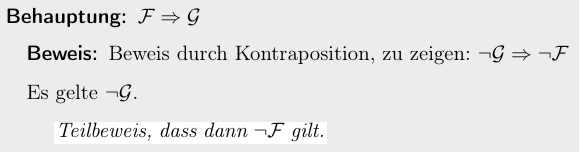
\includegraphics[width=0.6\textwidth, center]{./figures/kontraposition.png}

  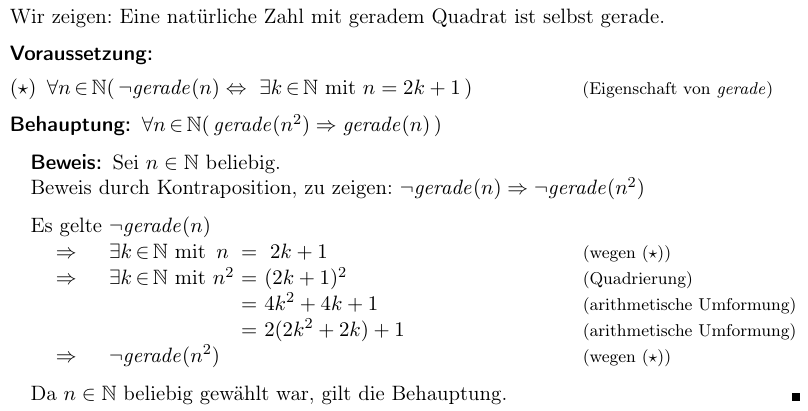
\includegraphics[width=0.8\textwidth, center]{./figures/kontraposition_example.png}
  \end{itemize}
\end{frame}

\begin{frame}[allowframebreaks]{Appendix}{Links}
  \begin{itemize}
    \item \url{https://www.mathematik.uni-marburg.de/~thormae/lectures/ti1/code/qmc/}
    \item \url{https://we.tl/t-xUFDLiFCyO}
    \item \url{https://we.tl/t-tnBjVtcgZH}
  \end{itemize}
\end{frame}
